\documentclass{article}
\usepackage{graphicx}

\title{Development of a Brittle Star Detection Model for NOAA Ocean Exploration Video Challenge}
\author{CrocoMarine ROV}
\date{\today}

\begin{document}
\maketitle

\section{Introduction}

This report details the development process of an AI model for detecting brittle stars in underwater video footage, as part of the 2024 NOAA Ocean Exploration Video Challenge.

\section{Project Overview}

This project aims to develop an AI model capable of accurately detecting brittle stars within underwater video footage. The model will be trained on a dataset of annotated images and videos, and its performance will be evaluated using relevant metrics. The success of this project will contribute to a more efficient and streamlined process for analyzing underwater video data, accelerating scientific discovery and understanding of marine ecosystems.

\section{Project Management}

To effectively manage the complexity of this project, we adopted a strategy of breaking down the main process into smaller, parallel tasks. This approach allowed for efficient allocation of resources and facilitated parallel progress across different aspects of the project. We utilized Jira, a project management tool, to track and coordinate these tasks, ensuring seamless collaboration among team members. The use of Jira proved highly beneficial for:

\begin{itemize}
    \item \textbf{Problem Decomposition:} Breaking down the main challenge into smaller, more manageable tasks facilitated a clearer understanding of the individual challenges and opportunities within the project.
    \item \textbf{Parallel Workflows:} Jira allowed us to effectively manage and track multiple tasks concurrently, enabling simultaneous progress on different aspects of the project.
    \item \textbf{Communication and Collaboration:} Jira served as a central hub for communication and collaboration, allowing team members to update progress, share ideas, and address issues in a transparent and efficient manner.
\end{itemize}

The next figure \ref{fig:jira_photo} illustrates the use of jira for project management.

\begin{figure}[htbp]
    \centering
    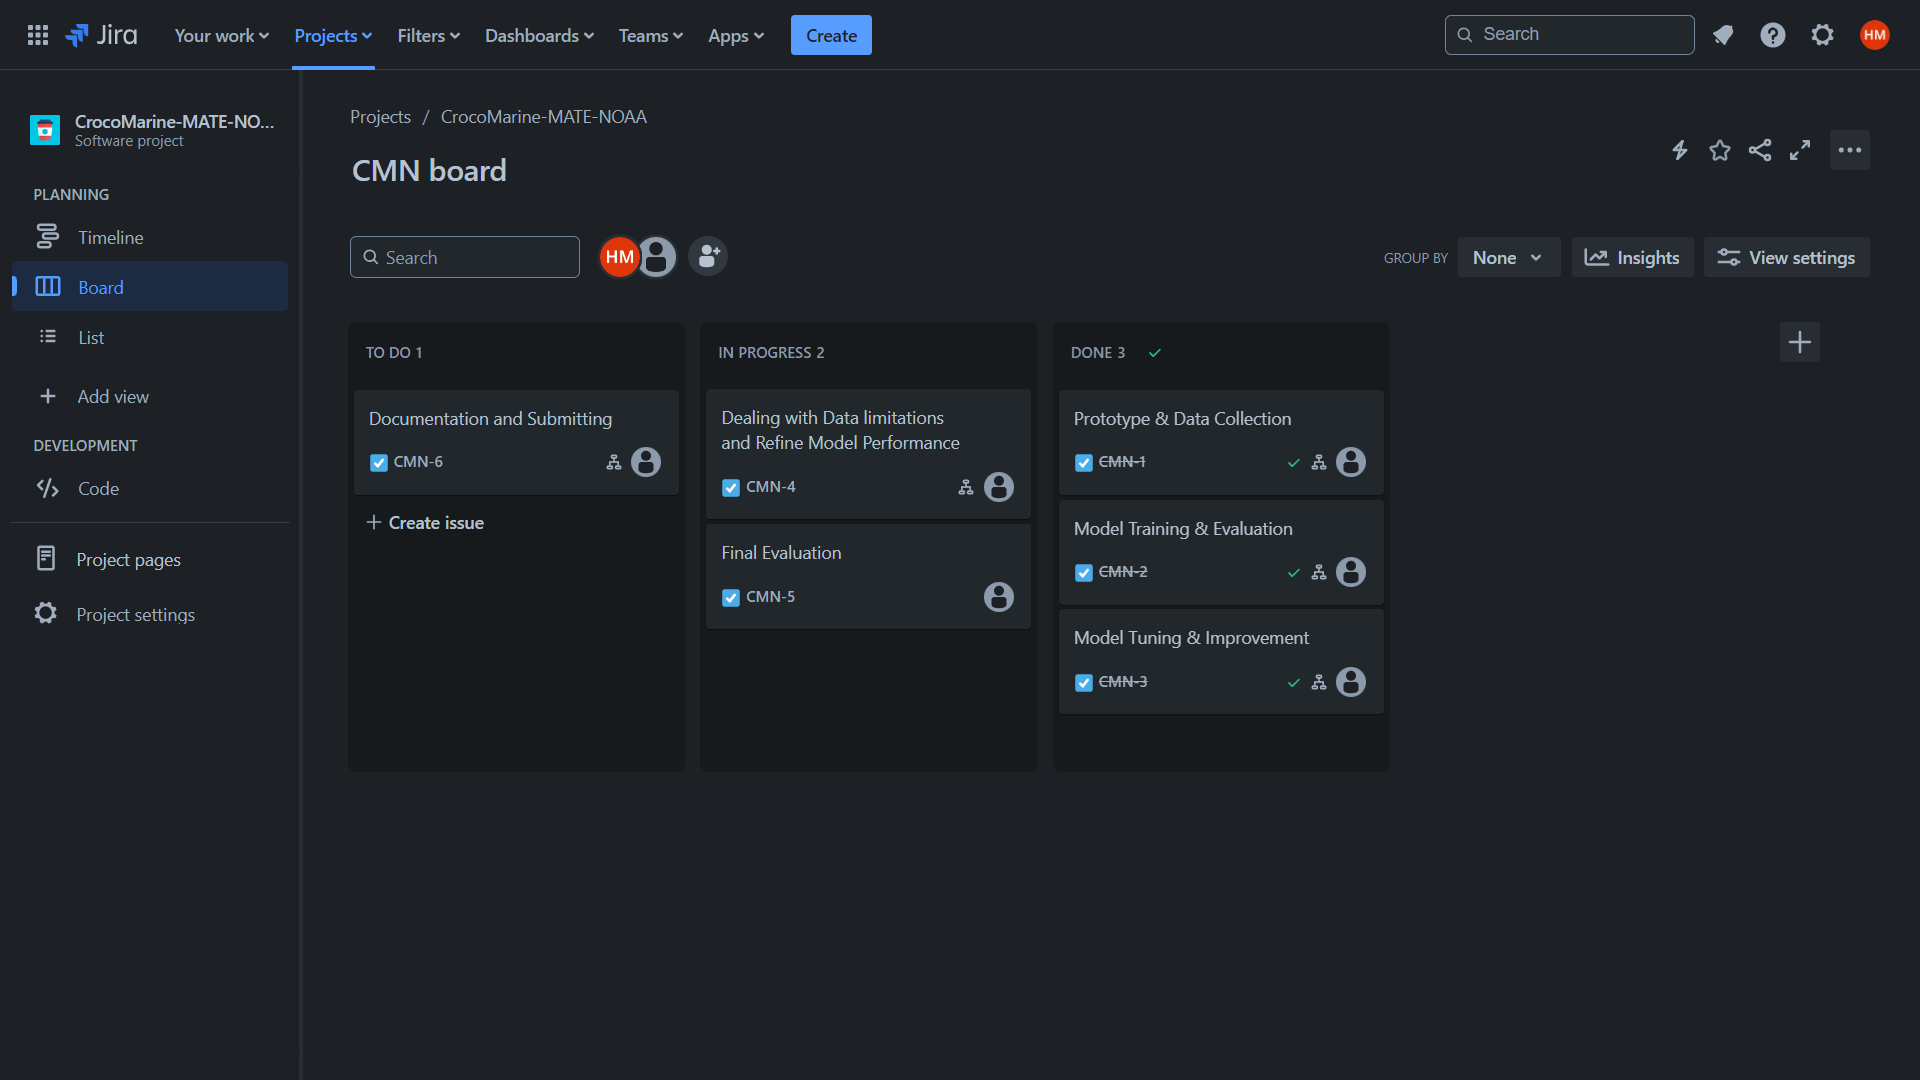
\includegraphics[width=0.8\textwidth]{jira.png}
    \caption{Jira Project Workflow.}
    \label{fig:jira_photo}
\end{figure}

\section{Project Workflow}

    The project workflow follows a Hybrid sequencential approach, where some tasks should be completed before moving on to the next, and Some can be done separately.\\
    The following figure \ref{fig:task_details} shows details about a random task where it is has child tasks, blocked by other tasks and blocks other tasks. \\
    This approach helped in organizing and working through the project efficiently.\\
    
    \begin{figure}[htb]
        \centering
        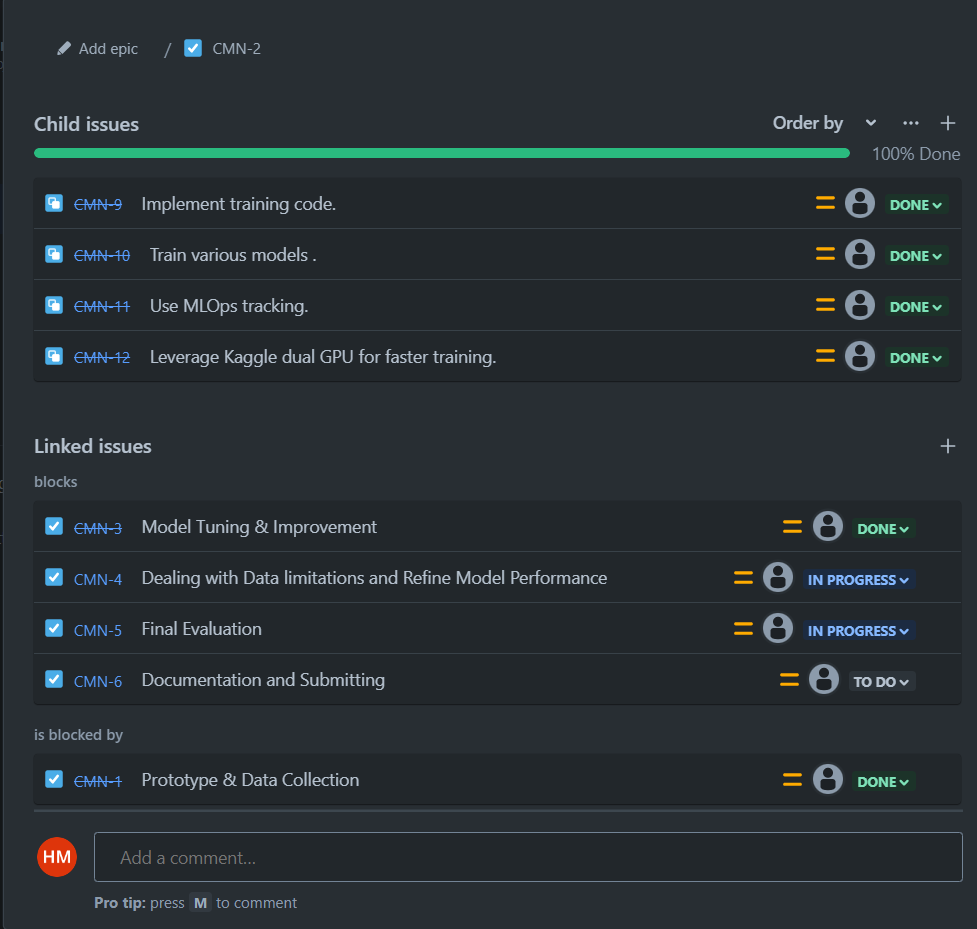
\includegraphics[width=0.8\textwidth]{process_image.png}
        \caption{Task details.}
        \label{fig:task_details}
    \end{figure}

    The following sections detail the development process of each task.
\subsection{Initial Model Development}

\subsubsection{Data Collection}

The project begained with the collection of an initial dataset to train a prototype model. This dataset consisted of images from publicly available sources.

\subsubsection{Data Annotation}

The collected data was annotated using Roboflow, a platform that simplifies the process of creating high-quality training datasets for object detection models. This involved drawing bounding boxes around each brittle star in the images.

\subsection{Model Training and Selection}

\subsubsection{Model Architecture}

Several popular object detection architectures were evaluated, including YOLOv8m, YOLOv8l, YOLONAS\_s, and YOLONAS\_m.

\subsubsection{Training Implementation}

Training code was implemented and executed using Kaggle dual GPU resources to accelerate the training process.

\subsubsection{Model Selection}

YOLOv8m was chosen due to its balance of efficiency and speed during training.

\subsection{Model Optimization and Evaluation}

\subsubsection{MLOps Tracking}

Weights \& Biases (WandB) was used to track model performance and experiments throughout the development process.\\

\subsubsection{Parameter Tuning}

Extensive tuning of hyperparameters was conducted, including:

\begin{itemize}
\item Batch Size: The Kaggle dual GPU platform enabled exploration of a wider range of parameter values, which gave The ability to tune batch size on different large values.
\item Learning Rate: Multiple learning rates were experimented with to achieve smooth and effective training.
\end{itemize}

The following figure shows the Tuning process for various models on Weights and Biases.
\begin{figure}[htb]
    \centering
    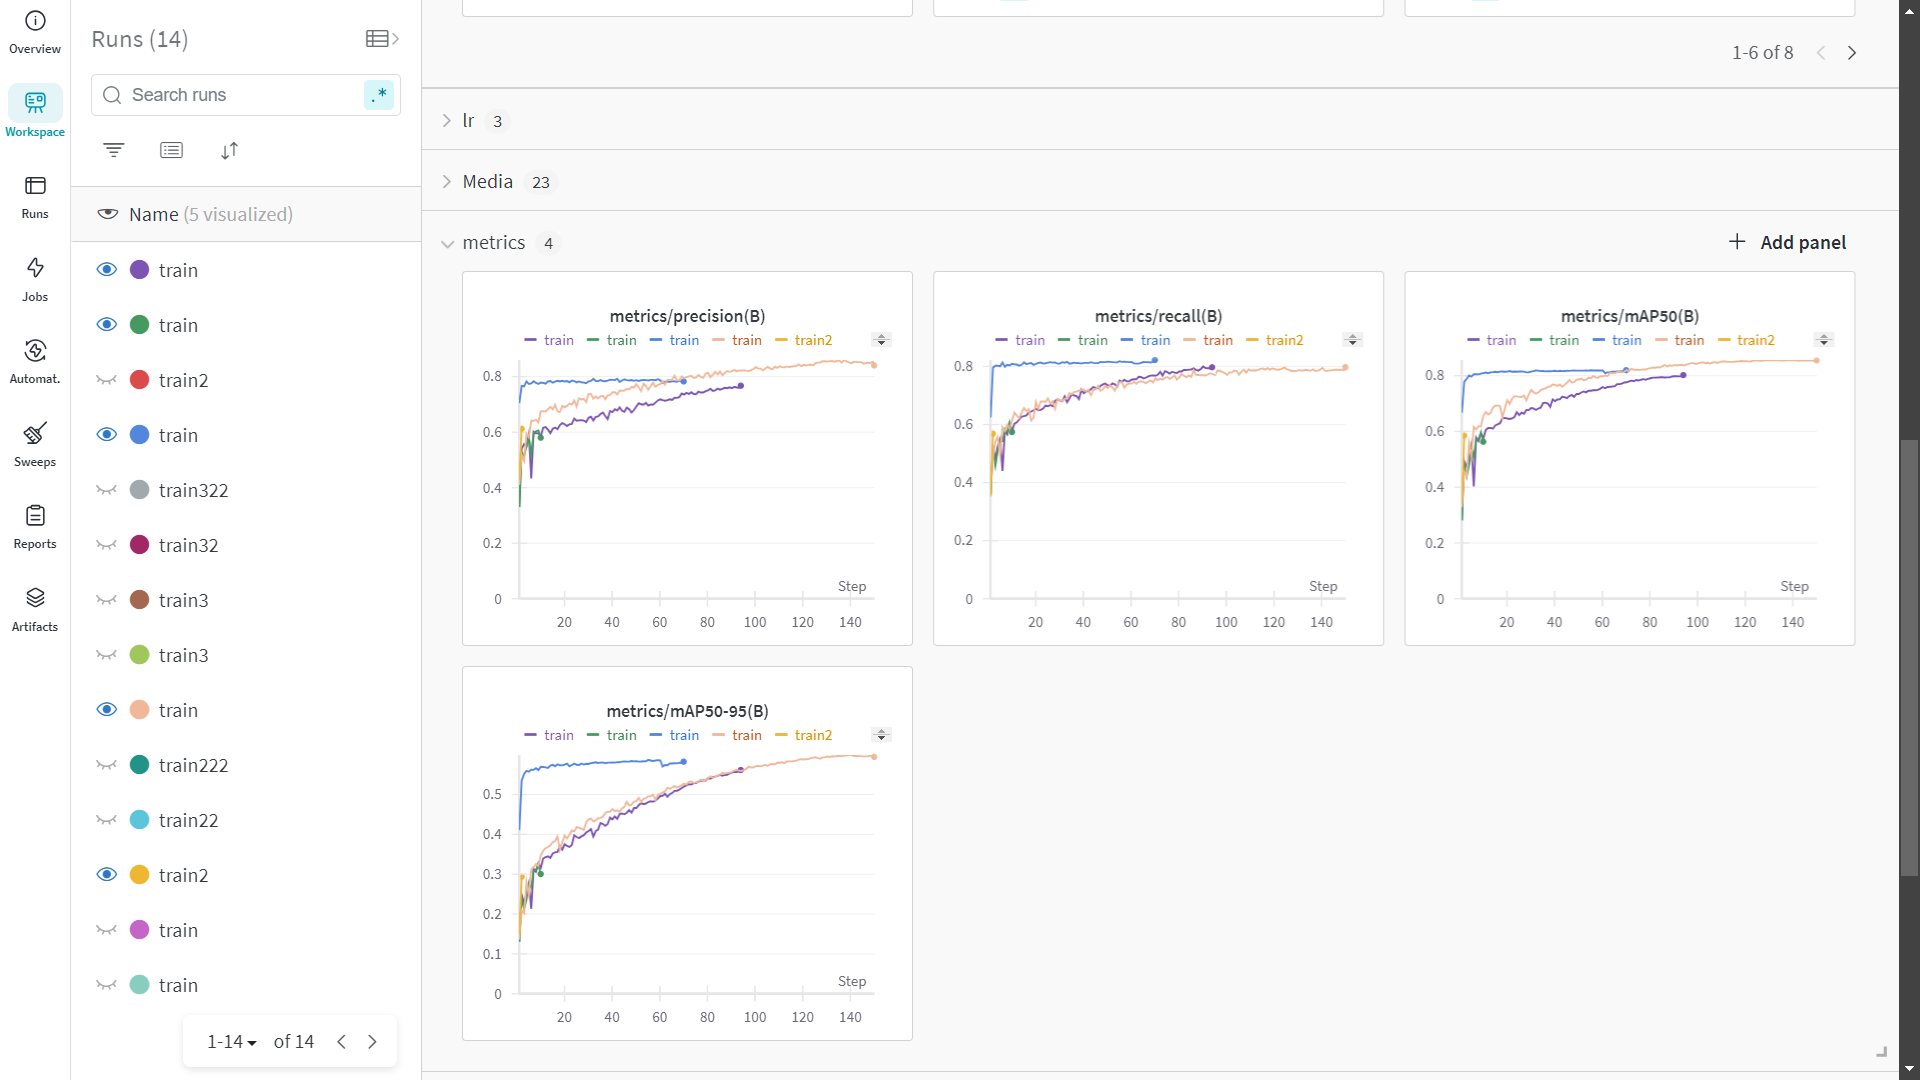
\includegraphics[width=0.8\textwidth]{wandb.png}
    \caption{Multiple models resuls on Weights and Biases.}
    \label{fig:wandb}
\end{figure}

\subsubsection{Metrics}

Model performance was evaluated using mean Average Precision (mAP) at thresholds of 50\% (mAP@50) and 50-95% (mAP@50-95).

\subsection{Addressing Model Errors}

\subsubsection{Data Validation}

Initial testing of the model on the video dataset revealed errors in the model's predictions. A review of the annotated data identified some inaccurate bounding boxes, leading to the correction of these annotations.

\subsubsection{Data Augmentation}

Additional data was collected and incorporated into the training dataset to enhance the model's performance.

\subsection{Enhancing Model Performance}

\subsubsection{Class Imbalance}

Due to limitations in finding suitable images online, it became clear that increasing the training data size was not feasible. To address this, a new class was introduced: "NOT BRITTLE STAR." This class taught the model to differentiate between the desired target (brittle star) and irrelevant objects. This simple step significantly improved the model's ability to identify the desired class.

\subsection{Final Model Performance}

After numerous training iterations and refinements, the model achieved satisfactory performance on the video dataset, demonstrating its ability to accurately detect brittle stars in the challenging underwater environment.

\subsection{Performance Comparison}
The table below illustrates the output metrics on the testing data usind various fine-tuned pre-trained models.\\
Its clear that YOLOv8m had the best trainig process so its used for further tuning achiving 0.65, 0.83 on mAP@50 and mAP@50-95.\\
\begin{table}[htb]
    \centering
    \begin{tabular}{|c|c|c|}
        \hline
        Model & mAP@50 & mAP@50-95 \\
        \hline
        YOLOv8m & 0.58 & 0.75\\
        YOLOv8l & 0.55 & 0.75\\
        YOLONAS\_m & 0.5 & 0.7\\
        YOLONAS\_m & 0.52 & 0.73\\
        \hline
    \end{tabular}
    \caption{Comparison of mAP scores for different models.}
    \label{tab:model_comparison}
\end{table}
\section{Conclusion}

This project successfully developed a robust and efficient AI model for identifying brittle stars in video footage. The use of Agile principles, including iterative development, constant evaluation, and adaptation to new information, played a crucial role in achieving this goal. This model has the potential to contribute to a more efficient and streamlined process for analyzing underwater video data, accelerating scientific discovery and understanding of marine ecosystems.

\end{document}
